\chapter{Clean Architecture}
\section{Was ist Clean Architecture?}
% allgemeine Beschreibung der Clean Architecture in eigenen Worten
Die Clean Architecture ist ein Architekturmuster, das sich auf die Trennung von Verantwortlichkeiten und die Abhängigkeiten zwischen den Schichten konzentriert. Die Architektur besteht aus mehreren Schichten, die von innen nach außen, wie in Abbildung \ref{fig:cleanArchitecture} zu sehen, angeordnet sind:

\begin{figure}[h]
    \centering
    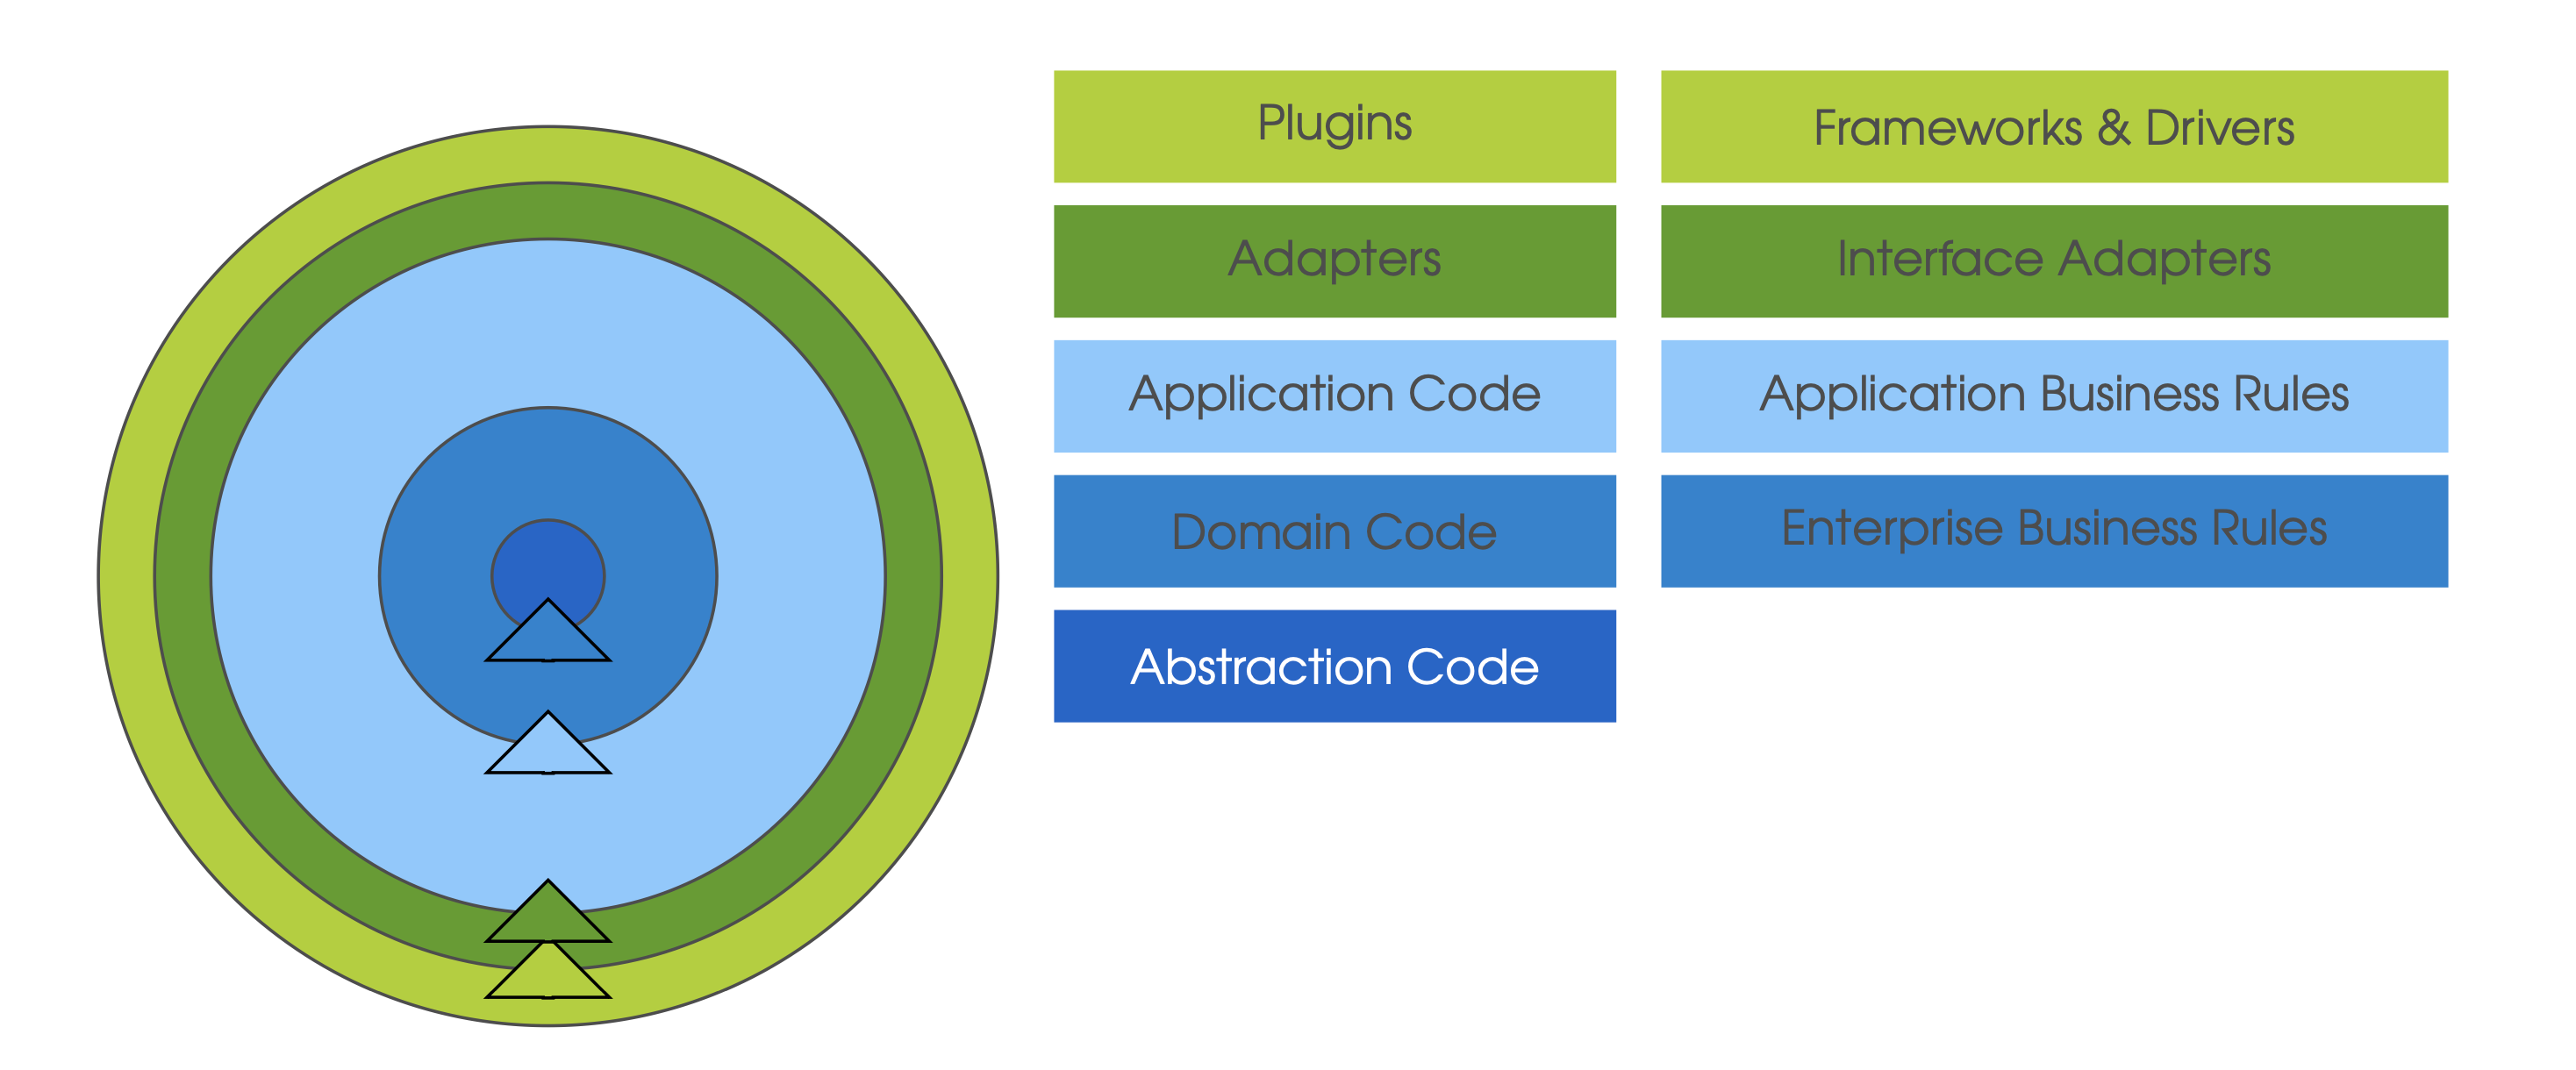
\includegraphics[width=0.8\textwidth]{Bilder/CA.png}
    \caption{Clean Architecture \cite{clean.2023}}
    \label{fig:cleanArchitecture}
\end{figure}

\begin{enumerate}
    \item \textbf{Abstraction Code (Schicht 4):} Code, welcher Konzepte, grundlegende Algorithmen und Datenstrukturen implementiert. Dieser Code enthält Domänen-übergreifendes Wissen und wird nur selten berührt.
    \item \textbf{Domain Code (Schicht 3):} Diese Schicht enthält die Kernlogik der Anwendung und wird am seltensten geändert. Hier werden die Geschäftsregeln und -modelle definiert. Die Entitäten der Domäne  werden von der Application Schicht verwendet.
    \item \textbf{Application Code (Schicht 2):} Diese Schicht enthält die Geschäftslogik der Anwendung(Use Cases welche direkt aus Anforderungen resultieren) und koordiniert den Datenfluss mit Hilfe der Entitäten der Domäne. Dabei sind die Regeln der anwendungsspezifischen Logik nicht projektweit gültig.  
    \item \textbf{Adapters (Schicht 1):} In der Adapter Schicht erfolgt die Kommunikation nach außen.Bei der Interaktion mit Plugins und anderen Anwendungen werden die von dort eingehenden Daten mit bereitgestellten Schnittstellen in interne Formate umgewandelt. Das primäre Ziel der Schicht ist die Entkopplung von innen und außen.
    \item \textbf{Plugins(Schicht 0):} Die Plugin Schicht interagiert grundsätzlich nur mit der Adapterschicht und enthält unter keinen Umständen Anwendungslogik. Als Beispiel sind an der Stelle Frameworks oder Benutzeroberflächen zu nennen.
\end{enumerate}

In der Betrachtung der Schichten von innen nach außen sei an der Stelle die Langlebigkeit des Codes erwähnt, welche nach außen hin abnimmt. Je weiter außen die Schicht liegt, desto häufiger wird sie geändert. Dabei weiß eine innere Schicht nichts von der äußeren, nur die äußere Schicht verwendet die innere. Das hat das Ziel, Code langlebiger zu machen und bei Änderungen der Technologien eine unveränderte Anwendung zu erhalten. 
\newpage
\section{Analyse der Dependency Rule}
% (1 Klasse, die die Dependency Rule einhält und eine Klasse, die die Dependency Rule verletzt);   jeweils UML der Klasse und Analyse der Abhängigkeiten in beide Richtungen (d.h., von wem hängt die Klasse ab und wer hängt von der Klasse ab) in Bezug auf die Dependency Rule
Im Projekt wurde dies konkret durch die Verwendung von Maven umgesetzt. Maven ist ein Build-Management-Tool, welches die Abhängigkeiten zwischen den einzelnen Schichten verwaltet. Es folgen zwei Beispiele, welche die Dependency Rule einhalten und verletzen.

\subsection{Positiv-Beispiel}
Als Positiv Beispiel sei an der Stelle die Klasse UserBuild eingeführt, wie in Abbildung \ref{fig:UserBuild} zu sehen. Die Klasse liegt in der Adapter Schicht, da sie die Aufgabe hat die jeweilige Simpsons-Figur der Wahl aus den inneren Schichten zu vermitteln. Verwendet wird die Klasse in der QuestionManager Klasse der Application Schicht. Dadurch bleiben die Abhängigkeiten von Adapters zu Application Code bis zu Domain Code, in dem die separaten Klassen der Simpsons Figuren liegen, erhalten.
\begin{figure}[ht]
    \centering
    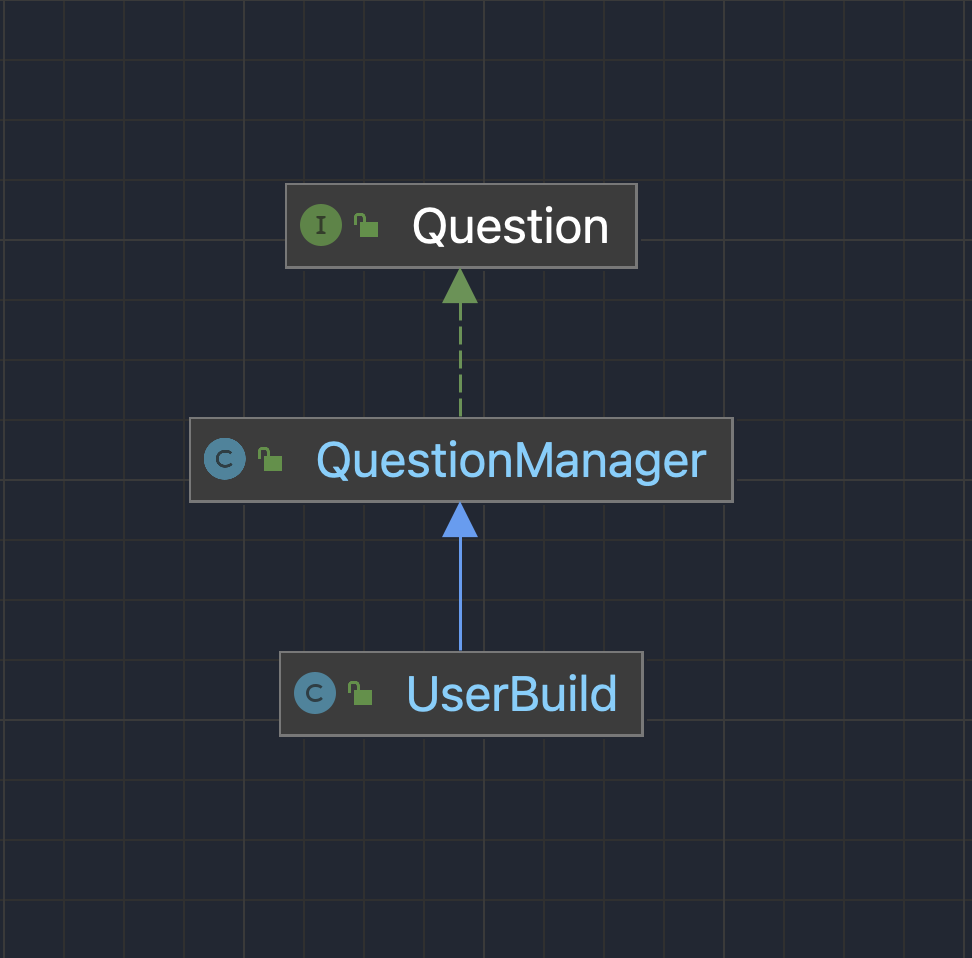
\includegraphics[width=0.4\textwidth]{Bilder/UserBuild.png}
    \caption{UML Klassendiagramm (UserBuild) Positiv Beispiel Dependency Rule}
    \label{fig:UserBuild}
\end{figure}
\newpage

\subsection{Negativ-Beispiel}
Ein Negativ Beispiel oder Verletzung der Dependency Rule lässt sich leider nicht zeigen, da die Dependency Rule in unserem Projekt nicht verletzt wurde. Dies liegt daran, dass die einzelnen Schichten durch Maven verwaltet werden und somit die Abhängigkeiten zwischen den einzelnen Schichten klar definiert sind. Listing \ref{code:pom} zeigt die Abhängigkeiten welche im \ac{POM} der Adapter Schicht festgelegt wurden.\newline
Ein mögliches Negativ Beispiel wäre, wenn zum Beispiel die Klasse Apu aus der Domain Schicht mit der introduce() Methode das Banner der GameTerminal Klasse verwenden würde. Dadurch würde ein Verstoß gegen die Dependency Rule vorliegen, da die Domain Schicht nicht auf die Adapter Schicht zugreifen darf. 

\lstinputlisting[
	label={code:pom},  % Label; genutzt für Referenzen auf dieses Code-Beispiel
	caption={Dependency Rule in der Adapter Schicht},  % Caption; genutzt für Referenzen auf dieses Code-Beispiel
	captionpos=b,               % Position, für die Caption:  t(op) oder b(ottom)
	style=EigenerABAPStyle,     % Eigener Style der vor dem Dokument festgelegt wurde
	firstline=1,                % Zeilennummer im Dokument welche als erste angezeigt wird
	lastline=5                 % Letzte Zeile welche ins LaTeX Dokument übernommen wird
]{Quellcode/pom.xml}
\newpage
\section{Analyse der Schichten}
% jeweils 1 Klasse zu 2 unterschiedlichen Schichten der Clean-Architecture: jeweils UML der Klasse (ggf. auch zusammenspielenden Klassen), Beschreibung der Aufgabe, Einordnung mit Begründung in die Clean-Architecture
In diesem Abschnitt werden zwei Klassen aus verschiedenen Schichten der Clean Architecture vorgestellt. 
\subsection{Domain Code: Apu}
Zunächst sei die Klasse Apu, wie in Abbildung \ref{fig:Apu} zu sehen, eingeführt.
\begin{figure}[ht]
    \centering
    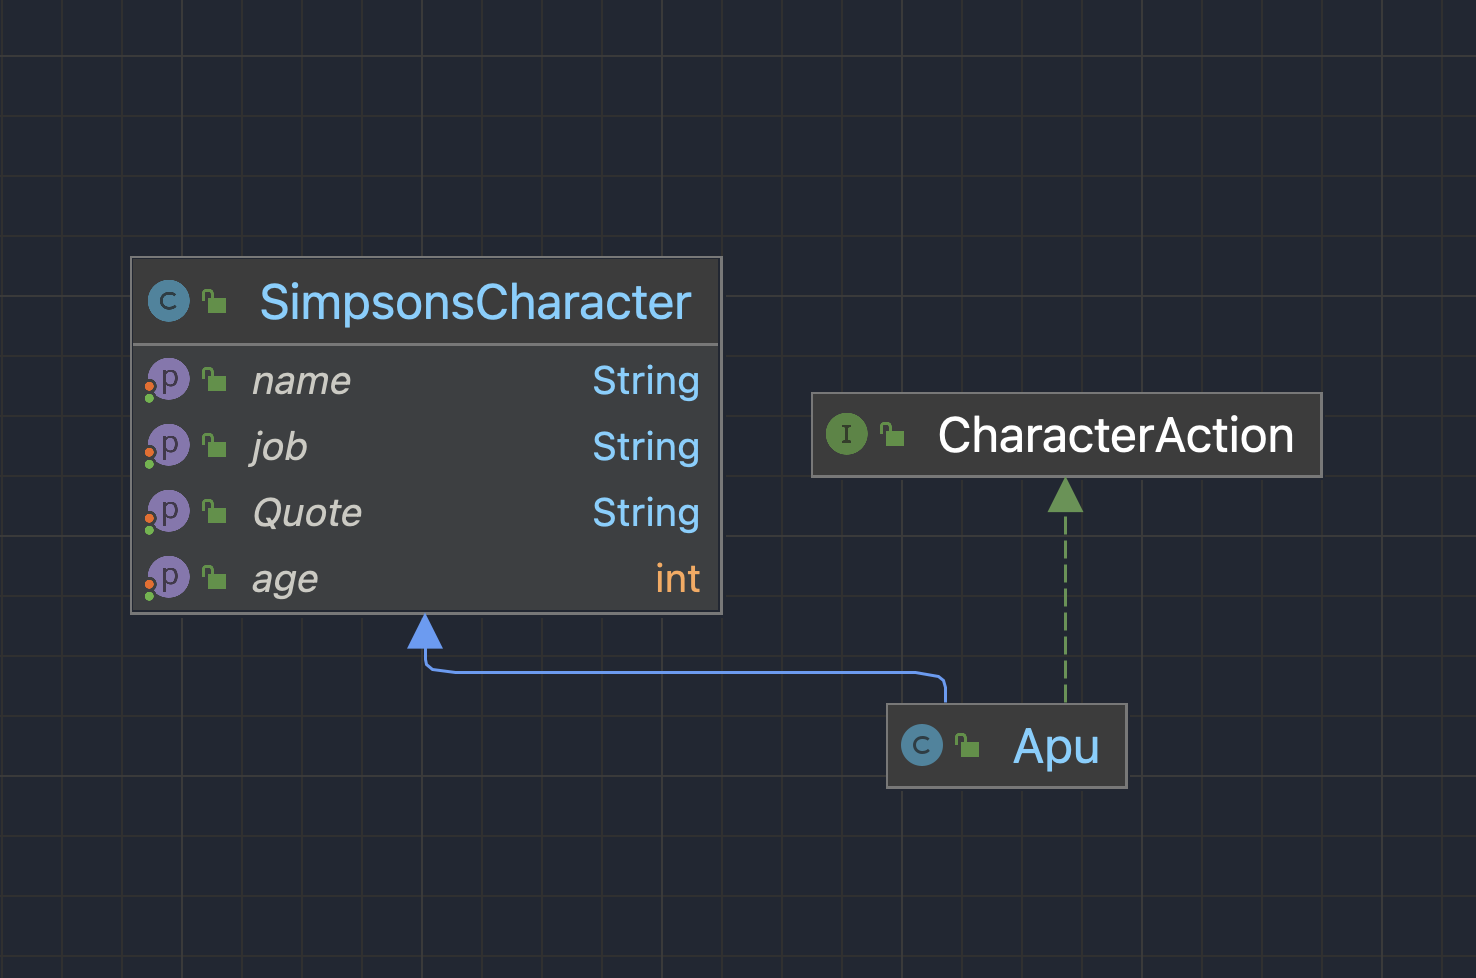
\includegraphics[width=0.4\textwidth]{Bilder/Apu.png}
    \caption{UML Klassendiagramm (Apu)}
    \label{fig:Apu}
\end{figure}
Die Klasse Apu ist eine Entität in der Domain Schicht und eine von 10 Figuren der Simpsons, welche in diesem Projekt implementiert wurden. Sie muss nicht angepasst werden, da sich die Eigenschaften einer Figur selten bis nie ändern. Sie wird dazu benutzt um im Verlauf des Quiz Ähnlichkeiten zum User aufzuzeigen und wird von der UserBuild Klasse im weiteren Spielverlauf verwendet.
\newpage
\subsection{Application Code: QuestionManager}
Die zweite Klasse ist die Klasse QuestionManager, wie in Abbildung \ref{fig:QuestionManager} zu sehen. Ihre Aufgabe ist die Verwaltung der Fragen und Antworten, welche im Quiz verwendet werden. Dabei enthält sie die notwendige Logik um basierend auf dem jeweiligen Use Case den entsprechenden Charakter zu ermitteln. Es besteht die Möglichkeit, dass die Klasse erweitert wird, da sich die Anforderungen an das Quiz im Laufe der Zeit ändern können.
\begin{figure}[ht]
    \centering
    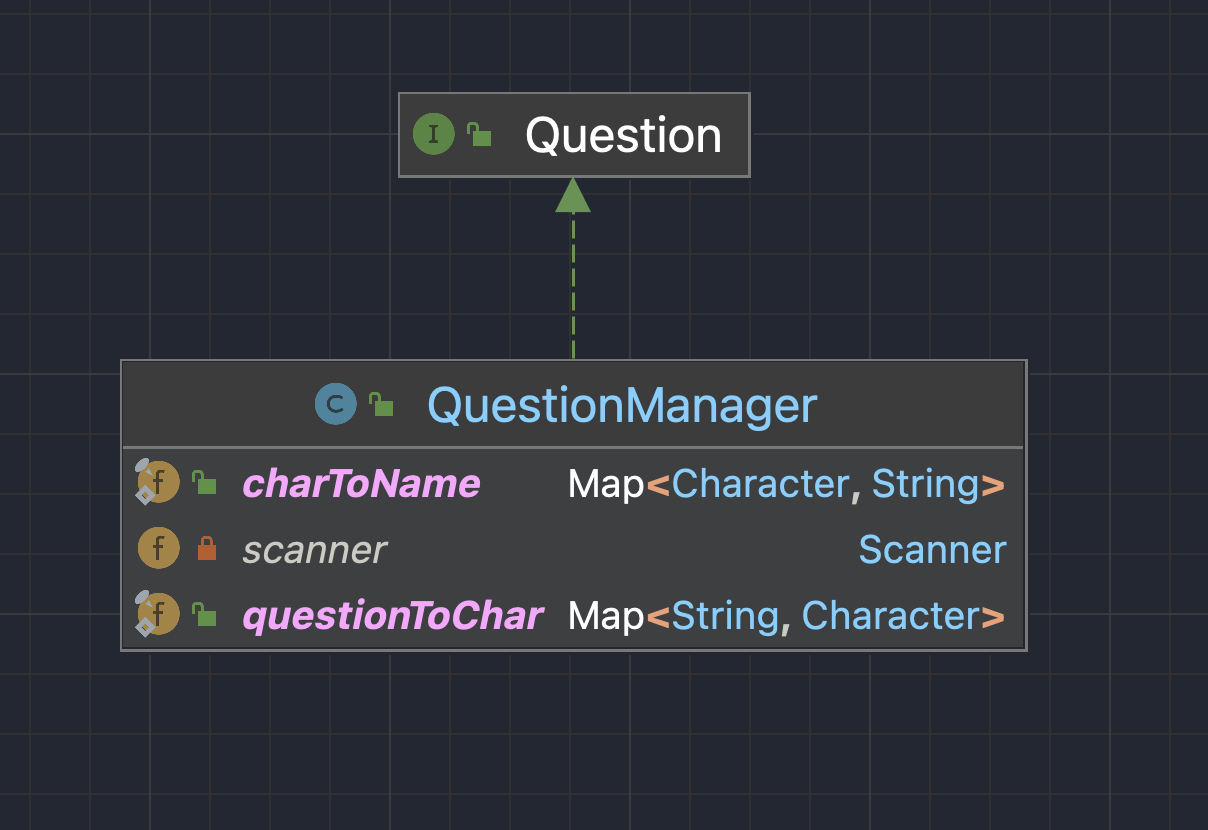
\includegraphics[width=0.4\textwidth]{Bilder/QM.png}
    \caption{UML Klassendiagramm (QuestionManager)}
    \label{fig:QuestionManager}
\end{figure}
